
%(BEGIN_QUESTION)
% Copyright 2010, Tony R. Kuphaldt, released under the Creative Commons Attribution License (v 1.0)
% This means you may do almost anything with this work of mine, so long as you give me proper credit

The {\it Pressure Swing Adsorption} (PSA) process uses a set of extremely fine filter elements called {\it molecular sieves} to ``strain'' nitrogen molecules from air, allowing oxygen and lighter gases to pass through:

$$\includegraphics[width=15.5cm]{i00056x01.eps}$$

A control system sequences the ball valves such that one vessel adsorbs (filters out nitrogen from air) while the other two regenerate (backflush with oxygen gas to purge out all the trapped nitrogen).

\vskip 10pt

Identify which valves are open and which valves are closed during the portion of the cycle where vessel A is adsorbing, and vessels B and C are both regenerating.  Trace the flow of air, oxygen, and (backwashed) nitrogen through all process lines.

\vfil 

\underbar{file i00056}
\eject
%(END_QUESTION)





%(BEGIN_ANSWER)

This is a graded question -- no answers or hints given!

%(END_ANSWER)





%(BEGIN_NOTES)

$$\includegraphics[width=15.5cm]{i00056x02.eps}$$

%INDEX% Final Control Elements, valve: packing
%INDEX% Process: pressure-swing-adsorption (PSA) production of oxygen

%(END_NOTES)


